% Owner: Hassan Ashraf 24L-3073
\section{Classical Models (Scikit-Learn)}
\label{sec:classical}

\subsection{Task and Framework Choice}

Deliverable 2 treats forecasting as a binary classification problem. For each
trading day the models predict \texttt{direction\_5d}: whether the gold price
will be higher five trading days later (1, ``up'') or not (0, ``down or
flat''). The input is one row of the features built in
Section~\ref{sec:features_eda}. Two feature sets are compared:
\textbf{all} (27 columns) and \textbf{stationary} (14 columns), which removes the
13 price-level columns such as \texttt{gold}, \texttt{gold\_lag5} and
\texttt{gold\_ma30} and keeps only returns, volatility, calendar terms and the
outlier flag.

We use \textbf{scikit-learn}~\cite{a_pedregosa2011} for the classical models
because the data is tabular and small (2,988 training rows), which is exactly
where linear models and tree ensembles are strong. Scikit-learn gives every
model the same \texttt{fit}/\texttt{predict\_proba} interface, provides
time-series cross-validation and grid search out of the box, and makes every
run reproducible through a fixed random seed (42). Its histogram-based gradient
boosting belongs to the same family as XGBoost~\cite{a_chen2016}, so no extra
library is needed. The deep-learning model (Section~\ref{sec:deep}) uses
PyTorch.

\subsection{Models}

\begin{itemize}
  \item \textbf{Majority baseline} (\texttt{DummyClassifier}): always predicts
        the most frequent class of the training set (``up''). Any useful model
        must beat it.
  \item \textbf{Logistic regression}: learns one weight per feature and turns
        the weighted sum into a probability with the logistic function. It can
        only draw a straight decision boundary, which makes it simple, stable
        and easy to interpret. The hyperparameter $C$ is the inverse of the L2
        regularisation strength.
  \item \textbf{Random forest}~\cite{a_breiman2001}: averages many decision
        trees, each trained on a bootstrap sample of the days and a random
        subset of the features. Averaging reduces the variance of single trees
        and captures non-linear interactions between features.
  \item \textbf{Histogram gradient boosting}~\cite{a_friedman2001}: builds
        shallow trees one after another, each correcting the errors of the
        previous ones. It is usually the strongest model on tabular data but
        also the easiest to overfit.
\end{itemize}

All models except the baseline use \texttt{class\_weight="balanced"}, so that
the slightly larger ``up'' class does not dominate training.

\subsection{Hyperparameter Tuning}

Each model is tuned with an exhaustive grid search
(\texttt{GridSearchCV}) on the training split only, scored by AUC-ROC. The
folds come from a walk-forward \texttt{TimeSeriesSplit} with five folds and a
gap of five days (Section~\ref{sec:evaluation}). Every grid is searched twice,
once per feature set, giving 90 configurations in total; all of them are saved
in \texttt{results/tuning/classical\_tuning.csv}.
Table~\ref{tab:classical-grid} lists the values tested and the reason for each
range.

\begin{table}[H]
  \centering
  \small
  \begin{tabular}{p{2.2cm}p{4.3cm}p{6.6cm}}
    \toprule
    Model & Values tested & Justification \\
    \midrule
    Majority & none & Fixed reference point \\
    Logistic regression & $C \in \{0.01, 0.1, 1, 10\}$ & From strong to weak regularisation, on a log scale \\
    Random forest & \texttt{n\_estimators} $\in \{200, 500\}$; \texttt{max\_depth} $\in \{3, 5, 8, \text{None}\}$; \texttt{min\_samples\_leaf} $\in \{1, 5, 20\}$ & More trees reduce variance; depth and leaf size control how closely each tree can fit noise \\
    Hist.\ gradient boosting & \texttt{learning\_rate} $\in \{0.03, 0.1\}$; \texttt{max\_depth} $\in \{3, 5\}$; \texttt{max\_iter} $\in \{200, 500\}$; \texttt{l2\_regularization} $\in \{0, 1\}$ & Small learning rates and shallow trees are the standard defence against overfitting noisy data \\
    \bottomrule
  \end{tabular}
  \caption{Hyperparameter grids for the classical models (16 to 24 configurations per tree model).}
  \label{tab:classical-grid}
\end{table}

\subsection{Final Choice}

For every model the configuration with the best mean cross-validation AUC was
kept for each feature set. The validation split (2022--2023) was then used once
to choose between the two feature sets. Table~\ref{tab:classical-selected}
shows the result.

\begin{table}[H]
  \centering
  \small
  \begin{tabular}{llccl}
    \toprule
    Model & Features & CV AUC (sd) & Val.\ AUC & Selected settings \\
    \midrule
    Logistic regression & all        & 0.534 (0.058) & \textbf{0.530} & $C = 0.01$ \\
                        & stationary & 0.491 (0.037) & 0.499 & \\
    Random forest       & all        & 0.543 (0.050) & \textbf{0.538} & 200 trees, depth 5, leaf 20 \\
                        & stationary & 0.491 (0.033) & 0.505 & \\
    Hist.\ grad.\ boost.\ & all      & 0.547 (0.035) & \textbf{0.524} & rate 0.03, depth 3, 200 iter. \\
                        & stationary & 0.499 (0.029) & 0.485 & \\
    Majority            & all        & 0.500 (0.000) & 0.500 & -- \\
    \bottomrule
  \end{tabular}
  \caption{Best configuration per model and feature set (CV: mean and standard deviation over 5 folds). Bold: selected.}
  \label{tab:classical-selected}
\end{table}

Three observations guided the final choice:

\begin{enumerate}
  \item \textbf{The signal is weak.} The best models reach a cross-validation
        AUC of only 0.53--0.55, three to five points above chance. Predicting
        the direction of a heavily traded market is hard, which is consistent
        with the efficient-market hypothesis~\cite{a_fama1970}.
  \item \textbf{Strong regularisation wins.} Every model selected the most
        conservative settings available: the smallest $C$, the largest leaf
        size and the shallowest boosting trees. With a weak signal, simpler
        models generalise better.
  \item \textbf{The full feature set was selected for every model}, because the
        stationary set scored at or below chance. The price-level columns
        therefore carry most of the usable information in the training
        period. As Section~\ref{sec:evaluation} shows, this choice has a cost:
        prices in the test period lie far outside the training range.
\end{enumerate}

On the validation split the random forest is the best classical model
(AUC 0.538). Gradient boosting had the best cross-validation score but dropped
to 0.524 on validation, a sign of mild overfitting to the training period.

\subsection{Feature Importance}

Figure~\ref{fig:feature-importance} shows the permutation
importance~\cite{a_breiman2001} of the selected random forest: the drop in
validation AUC when one feature is randomly shuffled. The most important
features are the levels of platinum, copper, silver and oil and the lagged gold
price. Even the most important feature changes AUC by less than 0.01, which
again shows how little predictable structure the data contains. The reliance on
price levels explains the behaviour of the tree models on the test set
(Section~\ref{sec:evaluation}).

\begin{figure}[H]
  \centering
  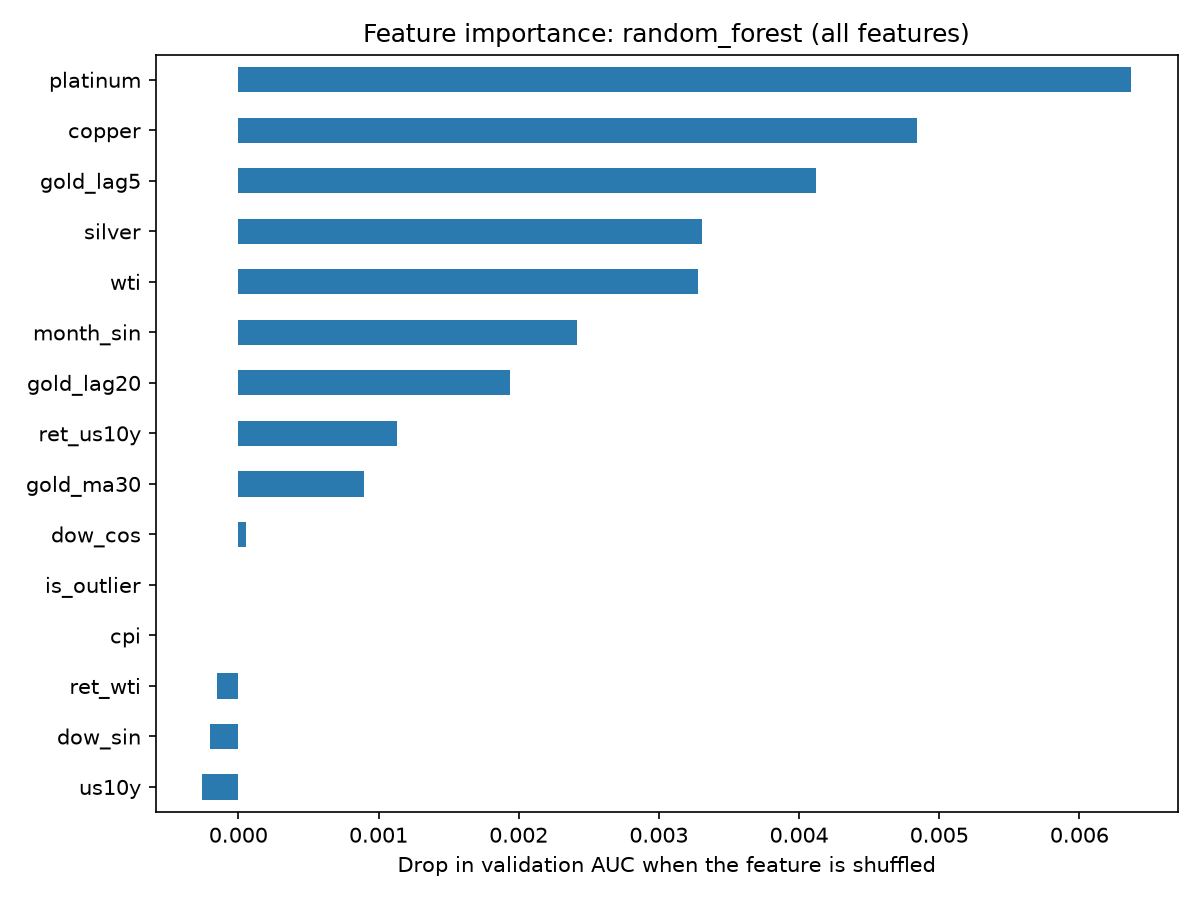
\includegraphics[width=0.75\textwidth]{classical/feature_importance.png}
  \caption{Permutation importance of the selected random forest on the validation split (top 15 features).}
  \label{fig:feature-importance}
\end{figure}